% 12 variables in here:
% u_1 = -1.0, h_1 = 10.0, U_1 = 0.0, H_1 = 10.0, u_2 = 0.0, h_2 = 10.0, U_2 = 0.0, H_2 = 10.0, u_3 = 0.0, h_3 = 10.0, U_3 = 0.0, H_3 = 10.0
\begin{figure}[h!]
\centering
  % \subfigure[Height and velocity for $p_1$] {
  %   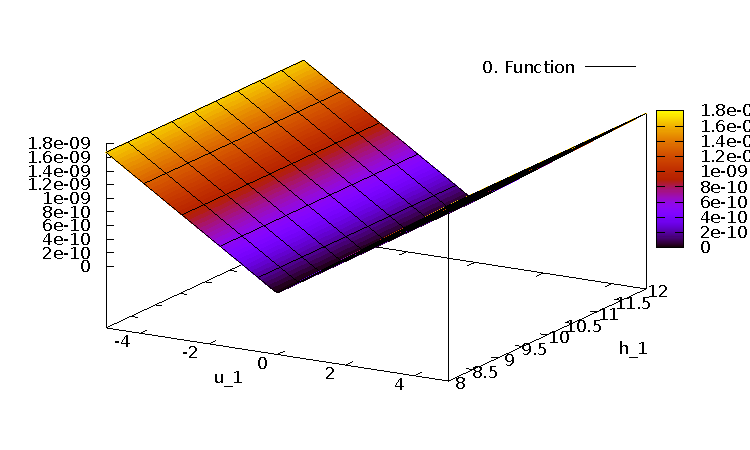
\includegraphics[scale=\zoomfactor]{{{3_punkte_1_impuls_verringert/x_y_0.0_10.0_0.0_10.0_0.0_10.0_0.0_10.0_0.0_10.0f0}}}  
  %   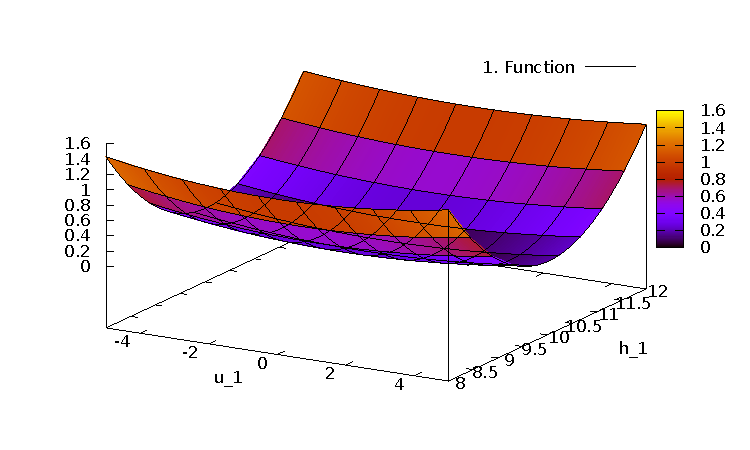
\includegraphics[scale=\zoomfactor]{{{3_punkte_1_impuls_verringert/x_y_0.0_10.0_0.0_10.0_0.0_10.0_0.0_10.0_0.0_10.0f1}}}  
  % }
  \subfigure[Height and velocity for $p_2^L$ resp. $p_2^R$] {
    \label{subfig:p2-height-impulse-three-points-p1-impulse-verringert}
    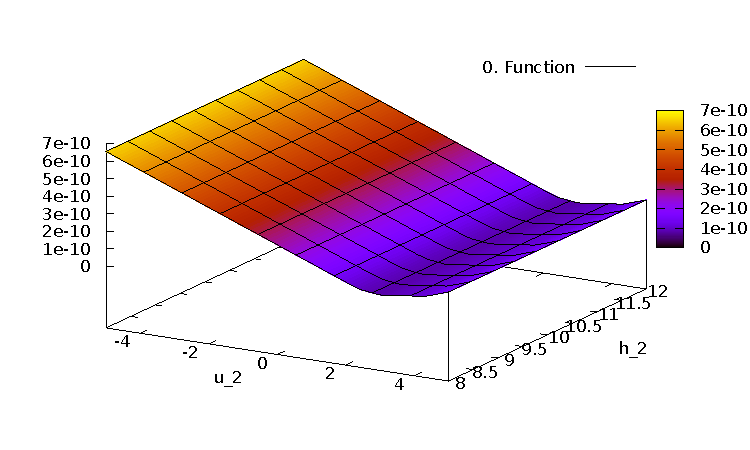
\includegraphics[scale=\zoomfactor]{{{3_punkte_1_impuls_verringert/-1.0_10.0_0.0_10.0_x_y_0.0_10.0_0.0_10.0_0.0_10.0f0}}}  
    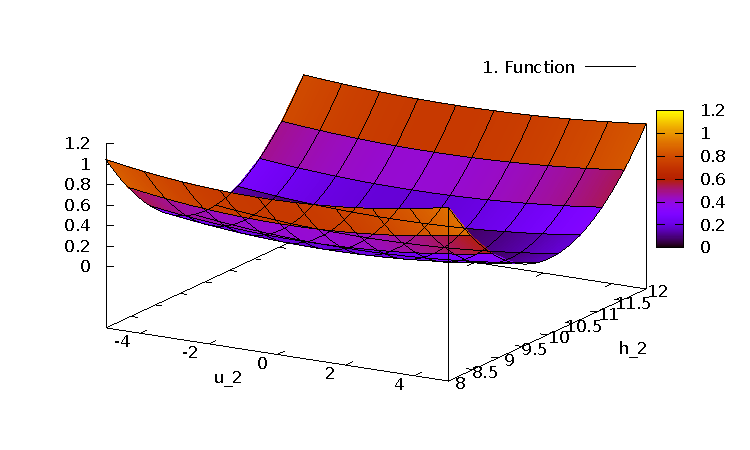
\includegraphics[scale=\zoomfactor]{{{3_punkte_1_impuls_verringert/-1.0_10.0_0.0_10.0_x_y_0.0_10.0_0.0_10.0_0.0_10.0f1}}}  
  }

  \subfigure[Height and velocity for $p_3^L$ res.p $p_3^R$] {
    \label{subfig:p3-height-impulse-three-points-p1-impulse-verringert}
    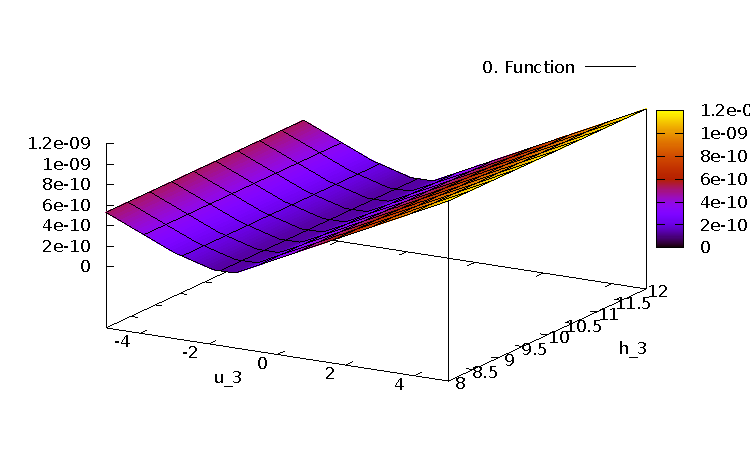
\includegraphics[scale=\zoomfactor]{{{3_punkte_1_impuls_verringert/-1.0_10.0_0.0_10.0_0.0_10.0_0.0_10.0_x_y_0.0_10.0f0}}}  
    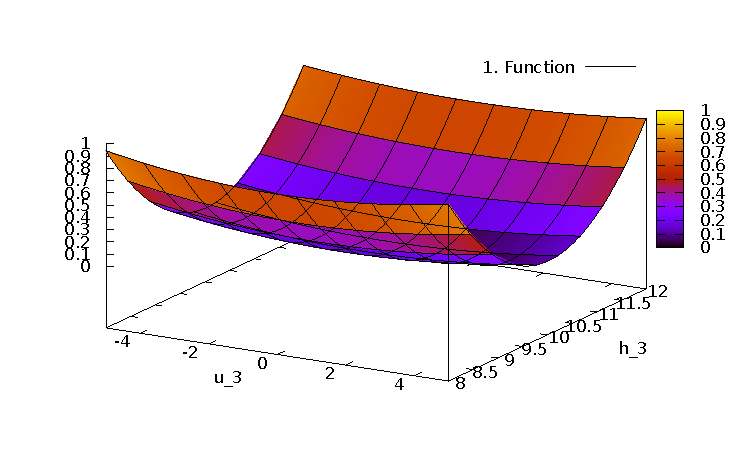
\includegraphics[scale=\zoomfactor]{{{3_punkte_1_impuls_verringert/-1.0_10.0_0.0_10.0_0.0_10.0_0.0_10.0_x_y_0.0_10.0f1}}}  
  }

  \subfigure[Height and velocity for $p_1^R$] {
    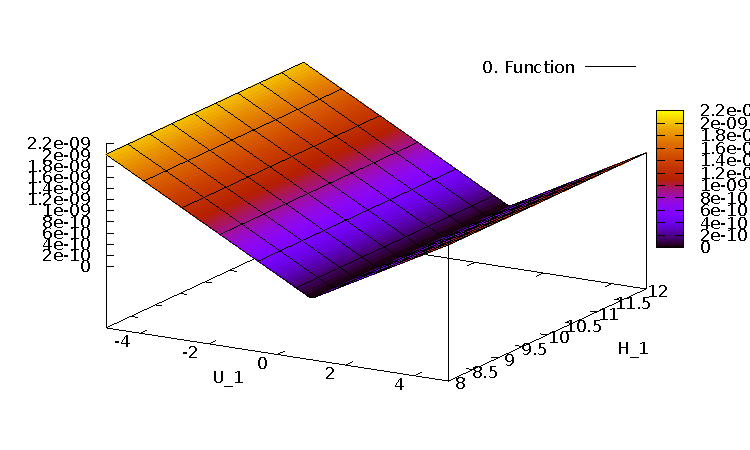
\includegraphics[scale=\zoomfactor]{{{3_punkte_1_impuls_verringert/-1.0_10.0_x_y_0.0_10.0_0.0_10.0_0.0_10.0_0.0_10.0f0}}}  
    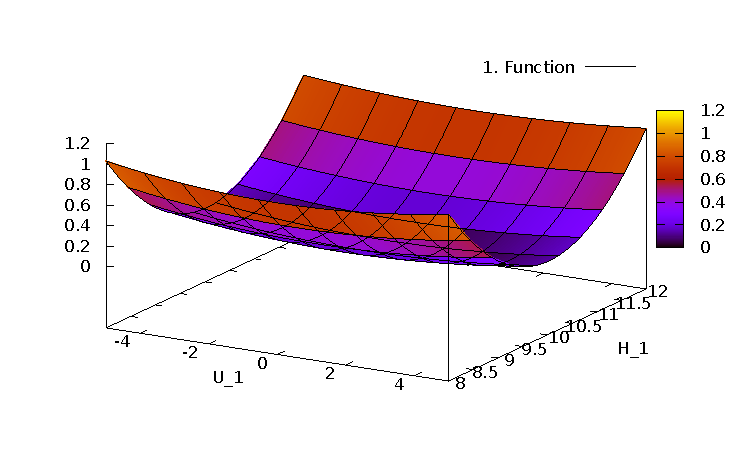
\includegraphics[scale=\zoomfactor]{{{3_punkte_1_impuls_verringert/-1.0_10.0_x_y_0.0_10.0_0.0_10.0_0.0_10.0_0.0_10.0f1}}}  
  }
  % \subfigure[Height and velocity for $p_2^R$] {
  %   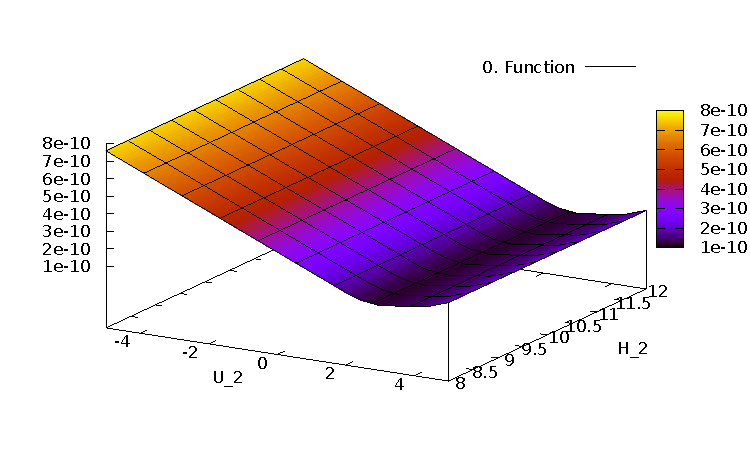
\includegraphics[scale=\zoomfactor]{{{3_punkte_1_impuls_verringert/-1.0_10.0_0.0_10.0_0.0_10.0_x_y_0.0_10.0_0.0_10.0f0}}}  
  %   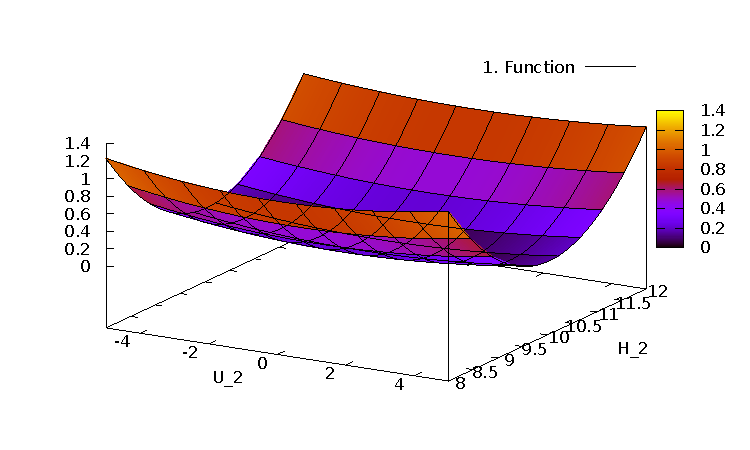
\includegraphics[scale=\zoomfactor]{{{3_punkte_1_impuls_verringert/-1.0_10.0_0.0_10.0_0.0_10.0_x_y_0.0_10.0_0.0_10.0f1}}}  
  % }

  % \subfigure[Height and velocity for $p_3^R$] {
  %   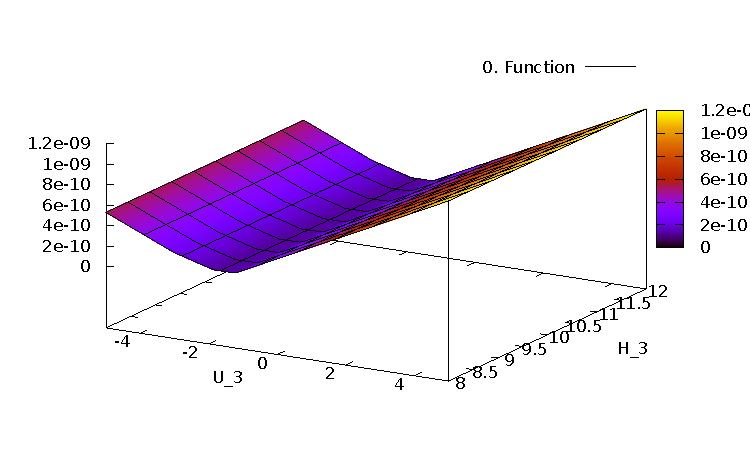
\includegraphics[scale=\zoomfactor]{{{3_punkte_1_impuls_verringert/-1.0_10.0_0.0_10.0_0.0_10.0_0.0_10.0_0.0_10.0_x_yf0}}}  
  %   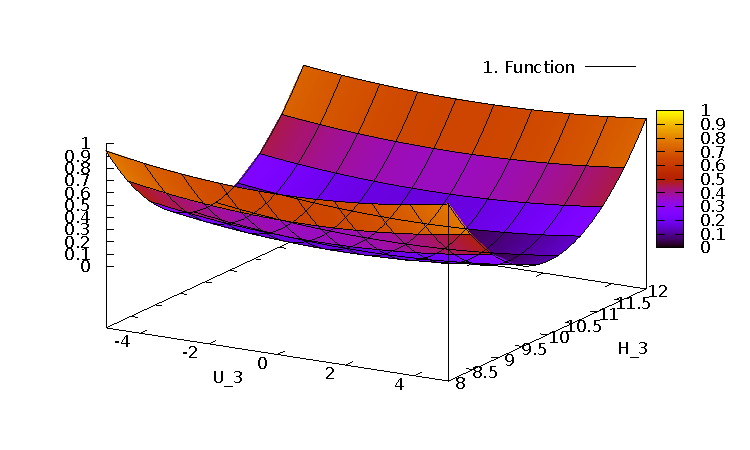
\includegraphics[scale=\zoomfactor]{{{3_punkte_1_impuls_verringert/-1.0_10.0_0.0_10.0_0.0_10.0_0.0_10.0_0.0_10.0_x_yf1}}}  
  % }
  \caption{Three points for each triangle. All points except $p_1$ have height 10, impulse 0. Point $p_1$ is set to $(10,-1)$. Surprisingly, changing the impulse results in  another error concerning the height component more than changing the height component. Subfigure \label{subfig:p2-height-impulse-three-points-p1-impulse-verringert} shows the height and impulse errors as well for $p_2^L$ and $p_2^R$ since the plots (at least) look so similar that they can't be distinguished with the naked eye. Moreover we sum up the plots for points $p_3^L$ and $p_3^R$ in subfigure \ref{subfig:p3-height-impulse-three-points-p1-impulse-verringert} for the same reason.
}
  \label{fig:three-points-u1-}
\end{figure}

%%% Local Variables:
%%% TeX-master: "../results.tex"
%%% End:
